\subsection{Recorded iterative WSP learning curves}\label{app:learning-curves}
The plots reconstruct all 174 trajectories from their original interaction records: 87 task, size and start settings in each information condition. Each selected training and development score agrees with the separately archived evaluator, and each final state agrees with the published endpoint. A rejected proposal leaves the selected weights unchanged. After early stopping, later opportunities display that retained state; they are not additional model calls. No new fitting or test-guided selection was performed for these plots. The data archive includes every selected state, all proposal decisions, raw and scaled errors, and exact counts.

Figure~\ref{fig:wsp-learning} uses the same scaled error as the main endpoint summary: divide each output error by the larger of one and the target magnitude before computing RMSE. It aggregates by the median over settings, not by first averaging within each task. No uncertainty band is drawn; these are descriptive summaries of the fixed cases. The median training error need not decrease because acceptance prioritizes development loss. The examples-only median development error falls from $0.0214$ to $5.89\times10^{-5}$, while the median training error rises from $9.03\times10^{-16}$ to $1.06\times10^{-3}$. Formula-and-examples medians change from $0.0248$ to $5.89\times10^{-5}$ on development and from $6.62\times10^{-16}$ to $1.32\times10^{-3}$ on training. The maximum of three attempted rounds does not establish convergence.

\begin{figure}[p]\centering
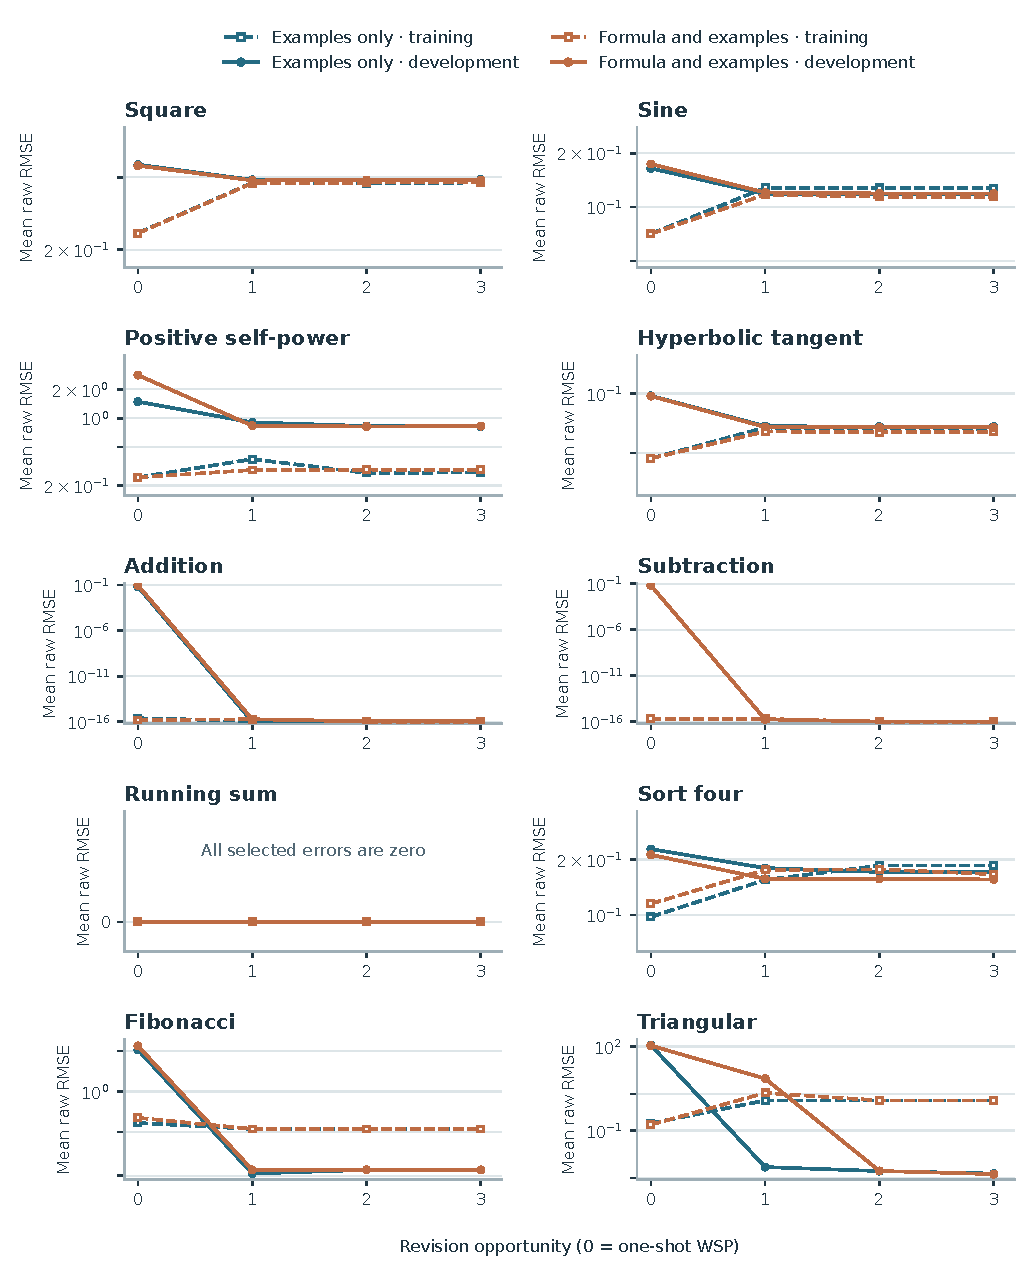
\includegraphics[width=\linewidth]{learning_tasks.pdf}
\caption{\textbf{Training and development curves for all ten tasks.} Each point is the mean raw RMSE over that task's tested sizes and three starts, using selected weights and carrying stopped states forward. Solid lines show development feedback; dashed lines show training. Colors distinguish examples only from formula and examples. Each task has its own logarithmic vertical range. Running sum is exact throughout and uses a linear axis at zero. Unlike the main learning curves, these within-task summaries use means, preserving the contribution of low-capacity networks that can be hidden by a zero median. The sorting panel reports errors across all output coordinates. Development data are reused for feedback and selection.}\label{fig:learning-tasks}
\end{figure}

\begin{figure}[p]\centering
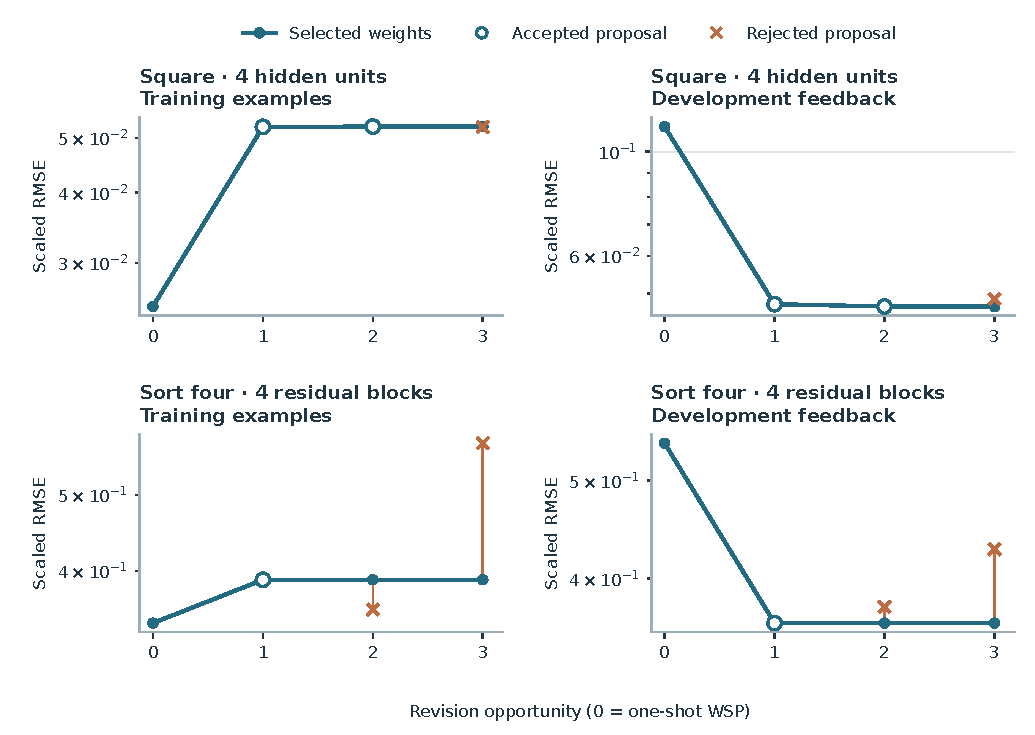
\includegraphics[width=\linewidth]{learning_proposals.pdf}
\caption{\textbf{A proposal is not necessarily the selected network.} Two illustrative examples-only trajectories at seed 164 show every valid proposal, the selected state, and training versus development scores. The square network has four hidden units; the sorting network has four residual blocks. Open circles mark accepted proposals and crosses mark rejected proposals. Vertical axes are logarithmic with separate ranges. Rejection leaves the selected curve flat. Selection minimizes scaled development loss first, using training loss only to break a tie. These examples explain selection behavior; Figure~\ref{fig:learning-tasks} covers the full task set.}\label{fig:learning-proposals}
\end{figure}
